\documentclass[]{bmcart}
\usepackage{lmodern}
\usepackage{amssymb,amsmath}
\usepackage{ifxetex,ifluatex}
\usepackage{fixltx2e} % provides \textsubscript
\ifnum 0\ifxetex 1\fi\ifluatex 1\fi=0 % if pdftex
  \usepackage[T1]{fontenc}
  \usepackage[utf8]{inputenc}
\else % if luatex or xelatex
  \ifxetex
    \usepackage{mathspec}
    \usepackage{xltxtra,xunicode}
  \else
    \usepackage{fontspec}
  \fi
  \defaultfontfeatures{Mapping=tex-text,Scale=MatchLowercase}
  \newcommand{\euro}{€}
\fi
% use upquote if available, for straight quotes in verbatim environments
\IfFileExists{upquote.sty}{\usepackage{upquote}}{}
% use microtype if available
\IfFileExists{microtype.sty}{%
\usepackage{microtype}
\UseMicrotypeSet[protrusion]{basicmath} % disable protrusion for tt fonts
}{}
\usepackage[margin=1in]{geometry}
\usepackage{longtable,booktabs}
\usepackage{graphicx}
\makeatletter
\def\maxwidth{\ifdim\Gin@nat@width>\linewidth\linewidth\else\Gin@nat@width\fi}
\def\maxheight{\ifdim\Gin@nat@height>\textheight\textheight\else\Gin@nat@height\fi}
\makeatother
% Scale images if necessary, so that they will not overflow the page
% margins by default, and it is still possible to overwrite the defaults
% using explicit options in \includegraphics[width, height, ...]{}
\setkeys{Gin}{width=\maxwidth,height=\maxheight,keepaspectratio}
\ifxetex
  \usepackage[setpagesize=false, % page size defined by xetex
              unicode=false, % unicode breaks when used with xetex
              xetex]{hyperref}
\else
  \usepackage[unicode=true]{hyperref}
\fi
\hypersetup{breaklinks=true,
            bookmarks=true,
            pdfauthor={},
            pdftitle={},
            colorlinks=true,
            citecolor=blue,
            urlcolor=blue,
            linkcolor=magenta,
            pdfborder={0 0 0}}
\urlstyle{same}  % don't use monospace font for urls
\setlength{\parindent}{0pt}
\setlength{\parskip}{6pt plus 2pt minus 1pt}
\setlength{\emergencystretch}{3em}  % prevent overfull lines
\setcounter{secnumdepth}{5}

%%% Use protect on footnotes to avoid problems with footnotes in titles
\let\rmarkdownfootnote\footnote%
\def\footnote{\protect\rmarkdownfootnote}

%%% Change title format to be more compact
\usepackage{titling}

% Create subtitle command for use in maketitle
\newcommand{\subtitle}[1]{
  \posttitle{
    \begin{center}\large#1\end{center}
    }
}

\setlength{\droptitle}{-2em}

  \title{}
    \pretitle{\vspace{\droptitle}}
  \posttitle{}
    \author{}
    \preauthor{}\postauthor{}
    \date{}
    \predate{}\postdate{}
  
\usepackage{booktabs}
\usepackage{longtable}
\usepackage{array}
\usepackage{multirow}
\usepackage{wrapfig}
\usepackage{float}
\usepackage{pdflscape}
\usepackage{tabu}
\usepackage{threeparttable}
\usepackage{threeparttablex}
\usepackage[normalem]{ulem}
\usepackage{makecell}

\usepackage{amsthm}
\newtheorem{theorem}{Theorem}[section]
\newtheorem{lemma}{Lemma}[section]
\theoremstyle{definition}
\newtheorem{definition}{Definition}[section]
\newtheorem{corollary}{Corollary}[section]
\newtheorem{proposition}{Proposition}[section]
\theoremstyle{definition}
\newtheorem{example}{Example}[section]
\theoremstyle{definition}
\newtheorem{exercise}{Exercise}[section]
\theoremstyle{remark}
\newtheorem*{remark}{Remark}
\newtheorem*{solution}{Solution}
\begin{document}



\begin{flushleft}
{\Large
\textbf\newline{DNA methylation modules associate with incident cardiovascular disease and cumulative risk factor exposure}
}
\newline
% Insert author names, affiliations and corresponding author email (do not include titles, positions, or degrees).
\\
Kenneth Westerman\textsuperscript{1},
Paola Sebastiani\textsuperscript{2},
Paul Jacques\textsuperscript{1},
Simin Liu\textsuperscript{3},
Dawn DeMeo\textsuperscript{4},
Jos\'e M. Ordov\'as\textsuperscript{1,5,6*}
\\
\bigskip
\textbf{1} JM-USDA Human Nutrition Research Center on Aging at Tufts University, Boston, MA, USA
\\
\textbf{2} Department of Biostatistics, Boston University School of Public Health, Boston, MA, USA
\\
\textbf{3} Department of Epidemiology, Brown University, Providence, RI, USA
\\
\textbf{4} Channing Division of Network Medicine, Department of Medicine, Brigham and Women's Hospital, Boston, MA, USA
\\
\textbf{5} IMDEA Alimentaci\'on, CEI, UAM, Madrid, Spain
\\
\textbf{6} Centro Nacional de Investigaciones Cardiovasculares (CNIC), Madrid, Spain
\\
\bigskip

* jose.ordovas@tufts.edu

\end{flushleft}

\section{Abstract}\label{abstract}

\textbf{Background} Epigenome-wide association studies using DNA
methylation have the potential to uncover novel biomarkers and
mechanisms of cardiovascular disease (CVD) risk. However, the direction
of causation for these associations is not always clear, and
investigations to-date have generally failed to replicate at the level
of individual loci. Here, we undertook module- and region-based DNA
methylation analyses of incident CVD in the Women's Health Initiative
(WHI) and Framingham Heart Study Offspring Cohort (FHS) in order to find
more robust epigenetic biomarkers for cardiovascular risk.

\textbf{Results} We applied weighted gene correlation network analysis
(WGCNA) and the Comb-p algorithm to find methylation modules and regions
associated with incident CVD in the WHI dataset. We discovered two
modules whose activation correlated with CVD risk and replicated across
cohorts. One of these modules was enriched for development-related
processes and overlaps strongly with epigenetic aging sites. For the
other, we showed preliminary evidence for monocyte-specific effects and
statistical links to cumulative exposure to traditional cardiovascular
risk factors. Additionally, we found three regions (associated with the
genes SLC9A1, SLC1A5, and TNRC6C) whose methylation associates with CVD
risk.

\textbf{Conclusions} In sum, we present several epigenetic associations
with incident CVD that reveal disease mechanisms related to development
and monocyte biology. Furthermore, we show that epigenetic modules may
act as a molecular readout of cumulative cardiovascular risk factor
exposure, with implications for the improvement of clinical risk
prediction.

\section{Introduction}\label{introduction}

Genetic approaches to cardiovascular disease (CVD) research have led to
important breakthroughs in mechanistic understanding and therapeutic
strategies. However, the mechanisms for gene variant-disease
relationships are often difficult to determine, and their effects may
often be mediated by epigenetic regulation {[}1{]}. DNA methylation is
one such mechanism that can reflect both genetic variation and
environmental exposures and potentially drive their effects on CVD
outcomes {[}2{]}.

A series of recent epigenome-wide association studies (EWAS) have
examined relationships between DNA methylation at
cytosine-phosphate-guanine (CpG) sites and various subtypes of CVD,
including prior myocardial infarction {[}3{]}, acute coronary syndrome
{[}4{]}, and atherosclerosis {[}5{]}. These cross-sectional studies may
reveal important mechanistic insights, but are susceptible to reverse
causation, i.e.~methylation being influenced by the presence of CVD.
Indeed, Mendelian randomization approaches across multiple phenotypes
have suggested that reverse causation is more common {[}6,7{]} than the
causal methylation effect that is often implicitly assumed. One approach
to this problem is to examine epigenetic associations with
cardiovascular risk factors. Multiple investigations have explored these
relationships genome-wide {[}8,9{]}, and have even uncovered prognostic
CpG sites for incident coronary heart disease in the process
{[}10,11{]}. A few studies looking directly at incident CVD as a binary
variable have found relationships with global DNA methylation (as
approximated by LINE-1 methylation levels) and with a specific cluster
of CpG sites in the ZBTB12 gene {[}12,13{]}.

Studies linking CVD and methylation have additionally shown a notable
lack of replication, especially at the level of single CpG sites
{[}14{]}. One approach to this problem is to aggregate CpGs and test
their phenotype associations at the group level. Differentially
methylated region (DMR) searches may improve detection by combining
sites based on physical proximity on the genome {[}15,16{]}. An
alternative grouping strategy is to search for correlation-based
clusters, which may boost biological signal and improve the
interpretability of results {[}17{]}. This approach was originally
developed for use with gene expression data, but has been successfully
applied to higher-dimensional DNA methylation microarray datasets
{[}18,19{]}.

To address the problem of reverse causation by CVD while achieving more
robust results, we set out to analyze relationships between group-level
CpG methylation and incident CVD using time-to-event models in two
cohorts. We used module- and region-based techniques to improve
detection and provide more interpretable results. We sought context for
two specific modules of interest using gene- and chromatin-based
annotations, and compared module activations to past and current
cardiovascular risk factor levels to better understand their potential
biological mechanisms.

\section{Results}\label{results}

\subsection{Weighted correlation network approach finds CVD-related
modules}\label{weighted-correlation-network-approach-finds-cvd-related-modules}

Population characteristics are described in Table 1. The discovery set,
Women's Health Initiative (n=2023), had a median age of 65 at blood draw
and is entirely female, while being selected for an approximately equal
ratio of subjects who did and did not experience an incident CVD event
following the methylation measurement timepoint. The replication set,
Framingham Heart Study Offspring Cohort (n=2587), had a median age of 66
at blood draw (Exam 8) and is approximately half female, with 305
subjects experiencing incident CVD events. Cardiovascular events were
defined here as encompassing coronary heart disease, stroke, and death
from CVD (see Methods section for further details).

\begin{table}

\caption{\label{tab:population-description}Population description}
\centering
\begin{tabular}[t]{lll}
\toprule
  & WHI & FHS\\
\midrule
Sample Size & 2023 & 2587\\
\% female & 100 \% & 55 \%\\
Age at blood draw & 65 (59-70) & 66 (60-73)\\
Mixed race & Yes & No\\
BMI & 29.1 (25.5-33.3) & 27.7 (24.5-31)\\
\addlinespace
\% smoke currently & 10\% & 9\%\\
Smoking pack-years & 0 (0-12.5) & 0 (0-0)\\
\# prior CVD events & 0 & 331\\
\# incident CVD events & 1009 & 305\\
\bottomrule
\multicolumn{3}{l}{\textsuperscript{1} Continuous values shown as: median (interquartile range).}\\
\multicolumn{3}{l}{\textsuperscript{2} 92 subjects experienced both prior and incident CVD events.}\\
\end{tabular}
\end{table}

We first set out to find biologically relevant modules in an
unsupervised manner (agnostic to incident CVD information) using the
WGCNA algorithm for 422952 CpGs in WHI passing quality control filters
(study overview in Supp. Fig. S1). After weighted correlation network
construction, topological overlap calculation, and subsequent
clustering, 110 modules were uncovered, ranging in size from 28 to 35361
CpGs.

Principal component eigenvectors for each module were calculated in
order to examine the characteristics of these modules as a whole. The
first principal component of each module tended to explain approximately
half of the total variance, while the rest contributed only small
fractions (see Supp. Fig. S2 for selected Scree plots). Thus, these
first eigenvectors, or ``eigenCpGs'', were subsequently used to describe
module behavior. Cox proportional hazards models were used to assess the
relationships between these module eigenCpGs and incident CVD. In
partially-adjusted models (adjusted for technical factors and estimated
white blood cell proportions), three modules were found to be associated
at multiple test-corrected FDR \textless{} 0.2 (Table 2; correction
based on 110 modules). Adjustment for biological covariates (age, BMI,
sex/race, and smoking behavior) attenuated these relationships to
marginal statistical significance (all 0.01 \textless{} p \textless{}
0.1; direct risk factor associations shown in Fig. 3). These modules
showed strong (FDR \textless{} 10\textsuperscript{-4}) enrichment for
different sets of GO terms, ranging from immune activation (myeloid or T
cell) to developmental processes.

\begin{table}

\caption{\label{tab:sig-module-table}Modules associated with incident CVD at FDR < 0.2}
\centering
\begin{tabular}[t]{lrrllll}
\toprule
\multicolumn{1}{c}{} & \multicolumn{1}{c}{} & \multicolumn{2}{c}{EigenCpG} & \multicolumn{3}{c}{Enrichment analysis} \\
\cmidrule(l{2pt}r{2pt}){3-4} \cmidrule(l{2pt}r{2pt}){5-7}
module & size & Var. expl. (\%) & p & GO terms & CpG Islands & Gene-based\\
\midrule
blue & 29441 & 44.61 & 0.00027 & Development & N\_shore & 1stExon/TSS/5' UTR\\
brown & 953 & 53.08 & 0.00455 & Immune activation & Open sea & \\
purple & 568 & 44.88 & 0.00500 & T cell activation & Open sea & Body\\
\bottomrule
\end{tabular}
\end{table}

All three modules showed very strong preservation in FHS (all
\(Z_{summary}\) statistics \textgreater{} 50, where 10 is a typical
threshold for strong preservation), when evaluated using established
density and connectivity preservation techniques {[}20{]}. Of these, two
associations with incident CVD (blue and brown) replicated strongly in
FHS, while purple showed nominal replication (p=0.0203) in
partially-adjusted models (Supp. Table 1). Fully-adjusted models
including age as a covariate attenuated (brown) or abolished (blue and
purple) these associations in FHS.

Though the existence of past CVD events (experienced prior to sample
collection for DNA methylation measurement) could represent a confounder
in the FHS dataset, sensitivity analyses adjusting for past events did
not appreciably reduce the strength of these module-trait relationships.
Also of potential relevance to this replication is the demographic
heterogeneity between the two cohorts. To address this possibility, we
performed additional analyses including interaction terms between
eigenCpGs for each module and either sex (in FHS) or race (in WHI). None
of these analyses produced significant interaction terms at p
\textless{} 0.05.

\subsection{Genome-wide associations between DNA methylation and
incident CVD
events}\label{genome-wide-associations-between-dna-methylation-and-incident-cvd-events}

To investigate more specific DNA methylation signals, we performed an
epigenome-wide association study (EWAS) for incident CVD. Of single
sites from the EWAS, 3 reached a genome-wide Bonferroni threshold, but
none replicated strongly in FHS (Supp. Table 2). In order to improve
statistical power, we focused on differentially methylated regions
(DMRs) with respect to incident CVD status. Single-site EWAS p-values
were used as input to the Comb-p algorithm, which seeks regions enriched
for low p-values while accounting for autocorrelation based on genomic
distance. Comb-p was applied separately to EWAS results from WHI and
FHS.

\begin{table}

\caption{\label{tab:combp-results}Comb-p regions with multiple test-corrected p<0.05 in WHI and Bonferroni p<0.05 in FHS}
\centering
\begin{tabular}[t]{lrlllll}
\toprule
\multicolumn{1}{c}{} & \multicolumn{1}{c}{} & \multicolumn{1}{c}{} & \multicolumn{1}{c}{} & \multicolumn{2}{c}{Discovery} & \multicolumn{1}{c}{Replication} \\
\cmidrule(l{2pt}r{2pt}){5-6} \cmidrule(l{2pt}r{2pt}){7-7}
Location & \# CpGs & Annotated gene & Genomic region & P & Adj. P & P\\
\midrule
chr1:27440462-27440721 & 3 & SLC9A1 & Body & 1.75e-08 & 2.85e-05 & 0.000103\\
chr19:47287777-47288263 & 6 & SLC1A5 & CpG shelf near TSS & 5.91e-07 & 0.000514 & 3.8e-10\\
chr17:76037034-76037562 & 6 & TNRC6C & CpG island in 5' UTR & 1.67e-05 & 0.013300 & 0.000189\\
\bottomrule
\end{tabular}
\end{table}

206 DMRs were found in WHI after Sidak multiple testing correction for
each DMR based on its length. Of these, 3 were both found in FHS and
replicated at a Bonferroni level (Table 3; Fig. 1). These regions were
annotated to two cellular transport genes (SLC9A1 and SLC1A5) and
TNRC6C, which codes for a scaffolding protein involved in miRNA-mediated
translational repression. Of the three WGCNA modules identified above,
brown CpG sites consituted part of 2 DMRs (at SLC9A1 \& SLC1A5), while
a single CpG from the blue module was also a member of the SLC9A1 DMR.

\subsection{Exploration of the brown and blue
modules}\label{exploration-of-the-brown-and-blue-modules}

Based on the results from the module- and region-centric analyses, we
investigated the brown and blue modules further for biological
significance. The brown module was associated with immune-related genes
as noted above, and was enriched strongly for ``open sea'' sites
(p=1.1e-42) and annotated enhancers (p=1.7e-33). In contrast, the blue
module was associated with development-related genes, and was enriched
moderately for sites near genic transcription start sites and strongly
for CpG islands (p \textless{} 2.2e-16) (Fig. 2a,b).

Given these observations, we examined relative enrichments of enhancer-
and promoter-associated histone marks across different blood cell
subtypes to better understand the cell type specificity of this signal.
Epigenetic peaks were annotated using data from the Roadmap Epigenomics
Project {[}21{]} and relative enrichments were calculated as the
fraction of module CpGs found in peaks divided by the fraction of all
CpGs found in peaks.

We observed the greatest enrichment of brown CpGs in 2
enhancer-associated chromatin annotations, DNase hypersensitivity sites
(DHS) and H3K4me1 histone peaks, from monocytes compared to other blood
cell subtypes (Fig. 2c). This could point towards monocyte-related
biology and inflammatory processes as an important shared mechanism for
cardiovascular risk between the two cohorts examined here. In contrast,
blue CpGs were enriched for DHS and promoter-associated H3K4me3 histone
peaks from hematopoietic stem cells (HSCs), providing a link to the
observed enrichment of develoment-related genes in this set.

The module CpG sets were also compared to two existing methylation-based
age predictors from Horvath and Hannum et al., as well as the recent
morbidity-directed phenoAge {[}22--24{]}. While enrichments for brown
CpGs were moderate to nonexistent, blue CpGs were strongly enriched for
all three of these sets, most highly for the original DNAm age developed
by Horvath (46/353; p=3.4e-5; hypergeometric test), despite the fact
that this model was developed based on only \textasciitilde{}21,000 CpGs
shared between multiple versions of the Illumina methylation microarray
platform. Furthermore, 28 of these 46 CpGs had associated positive
coefficients in the DNAm age predictor. This subset has been previously
observed to contain a disproportionate amount of Polycomb-group target
genes, which are known to associate with developmental processes and to
be generally hypermethylated with age {[}25{]}. Using SUZ12 binding
regions {[}26{]} as a proxy for Polycomb-group targets, we confirmed
their enrichment in the blue module (p = 1.37e-07). Surprisingly, the
blue eigenCpG showed only a modest correlation with age (r=0.09).

\subsection{Module-risk factor
relationships}\label{module-risk-factor-relationships}

Next, we examined correlations between these module eigenCpGs and
traditional cardiovascular risk factors. Though no extremely strong
module-risk factor correlations were observed (all
\textbar{}r\textbar{}\textless{}0.25), they tended to be stronger for
the brown module, especially in FHS (Fig. 3a). Age showed the greatest
association, while lipid and glycemic parameters also showed moderate
associations. To further probe relationships between the brown module
and risk factors in FHS, we retrieved historical risk factors measured
in previous Offspring Cohort exams. Visual inspection revealed a notably
stronger correlation between the module eigenCpG and cumulative (mean of
all previous exams) compared to current risk factor exposure. This
pattern applied for systolic blood pressure (strongly), triglycerides,
glucose, BMI, and LDL (which correlated in the ``expected'' direction
cumulatively, but non-intuitively at Exam 8) (Fig. 3b).

To better investigate this phenomenon, we tested associations between
the brown module and each of the cumulative risk factors after
adjustment for potential confounders. Specifically, for each risk
factor, linear models were used to predict the brown eigenCpG value
from either the current or cumulative risk factor level while adjusting
for the full set of EWAS covariates other than BMI (age/sex/smoking/cell
counts/study center/7 ctrl-probe PCs). Only for the brown module did
cumulative risk factor exposure show strong associations, which were
generally equal to or stronger than those of the current risk factors,
most notably for BMI, hsCRP, and triglycerides (Table 4). Though more
recent medication use could possibly explain discrepancies between
biological relationships with current and past risk factors, adjustment
for hypertension and lipid medication use did not notably affect the
results of these models.

\begin{ThreePartTable}
\begin{TableNotes}
\item[1] Regression results are presented as: beta (p-value).
\item[2] Models are adjusted for age, sex, smoking status and pack-years, estimated cell counts, study center, and 7 control probe principal components.
\end{TableNotes}
\begin{longtabu} to \linewidth {>{\raggedright}X>{\raggedright}X>{\raggedright}X>{\raggedright}X>{\raggedright}X}
\caption{\label{tab:cumulative-adjusted}Module-risk factor relationships (current and cumulative) after adjustment for covariates}\\
\toprule
\multicolumn{1}{c}{} & \multicolumn{2}{c}{brown} & \multicolumn{2}{c}{blue} \\
\cmidrule(l{2pt}r{2pt}){2-3} \cmidrule(l{2pt}r{2pt}){4-5}
Risk factor & Current & Cumulative & Current & Cumulative\\
\midrule
bmi & 0.036 (4.3e-06) & 0.051 (2.3e-10) & 0.026 (0.0061) & 0.019 (0.051)\\
glu & 0.021 (0.011) & 0.027 (0.0011) & -0.00065 (0.95) & -0.0045 (0.66)\\
hscrp & 0.021 (0.0077) & 0.039 (1e-06) & 0.025 (0.011) & 0.014 (0.15)\\
tg & 0.018 (0.02) & 0.042 (5e-07) & 0.021 (0.03) & 0.015 (0.14)\\
hdl & -0.021 (0.015) & -0.017 (0.056) & -0.038 (0.00031) & -0.03 (0.0067)\\
\addlinespace
ldl & -0.012 (0.13) & 0.0089 (0.29) & -0.00072 (0.94) & 0.027 (0.0088)\\
chol & -0.014 (0.11) & 0.019 (0.021) & -0.013 (0.2) & 0.012 (0.24)\\
sbp & 0.012 (0.15) & 0.024 (0.0084) & -0.011 (0.27) & -0.0015 (0.89)\\
\bottomrule
\insertTableNotes
\end{longtabu}
\end{ThreePartTable}

Finally, we used the basic mediation approach of Baron and Kenny
{[}27{]} to test whether brown module activation may mediate a portion
of the effects of cumulative risk factor exposure on cardiovascular
risk. A series of Cox models were created in FHS for these three most
strongly-associated risk factors (BMI, hsCRP, and triglycerides).
Covariates in all models included current values for the risk factor in
question, as well as technical factors, estimated cell counts, age, and
sex. Current risk factors did not show notable relationships with
incident CVD in any of the models. Having established the
exposure-mediator relationships (Table 4), we tested the association
with CVD risk of 1) cumulative risk factors, 2) module eigenCpGs, and 3)
both quantities together (Table 5; example causal diagram using hsCRP in
Supp. Fig. S4). In general, the significance of the module relationships
with CVD tended to decrease in the presence of cumulative risk factor
values. This fits with a model in which, rather than mediating
cardiovascular risk, module activation acts as a biomarker for the
actions of cumulative risk factor exposures by some other mechanism. As
only subjects with current risk factor values were included in each
model, sample sizes were largely identical across models.

\begin{table}

\caption{\label{tab:module-mediation}CVD risk models using cumulative risk factor exposure and brown module activation}
\centering
\begin{tabular}[t]{lllll}
\toprule
\multicolumn{1}{c}{} & \multicolumn{1}{c}{Risk factors only} & \multicolumn{1}{c}{Brown only} & \multicolumn{2}{c}{Full model} \\
\cmidrule(l{2pt}r{2pt}){2-2} \cmidrule(l{2pt}r{2pt}){3-3} \cmidrule(l{2pt}r{2pt}){4-5}
Risk factor & Cumulative & Module & Cumulative & Module\\
\midrule
bmi & 0.061 (0.009) & 0.012 (0.1) & 0.057 (0.015) & 0.01 (0.16)\\
hscrp & 0.64 (<0.001) & 0.014 (0.054) & 0.62 (<0.001) & 0.012 (0.12)\\
tg & 1.7 (<0.001) & 0.016 (0.039) & 1.7 (<0.001) & 0.012 (0.1)\\
\bottomrule
\multicolumn{5}{l}{\textsuperscript{1} Regression results are presented as: beta (p-value).}\\
\end{tabular}
\end{table}

\section{Discussion}\label{discussion}

Here, we performed a primarily module-based epigenetic analysis of
incident cardiovascular events in order to find robust, prospective
biomarkers and uncover novel mechanisms contributing to disease risk. We
began by constructing correlation-based clusters in the methylation data
from WHI using the WGCNA algorithm. This network-based feature
clustering approach can potentially improve the signal-to-noise ratio of
high-dimensional DNA methylation data while facilitating more clear
biological interpretation of results {[}28{]}. As WGCNA does not
consider class labels (i.e.~incident CVD status), the 110 modules
uncovered were not \emph{a priori} expected to be related to CVD and
rather reflected unbiased patterns in the data. After correction for
multiple testing, the first principal components (eigenCpGs) of three of
these modules were found to be related to incident cardiovascular
events. A gene ontology-based enrichment analysis of the genes annotated
to these modules found strong enrichment for either immune-related or
development-related processes. The finding of immune-related processes
is intuitive given that DNA from blood measures primarily immune cells,
while the development-related enrichment could possibly reflect
influences during early life {[}29{]}. Notably, these two module
``types'' (immune and development) have been uncovered in a prior
network-based DNA methylation analysis related to asthma {[}19{]},
suggesting that similar module types are a potentially general feature
of blood-based methylation patterns and that these patterns may not be
fully cardiovascular-specific, reflecting instead a predisposition
toward general inflammatory disease processes. Both in WHI and in
replication in FHS, two modules (blue and brown) showed strong
relationships with incident CVD that were attenuated after adjustment
for age (direct correlations of these modules with age are presented in
Fig. 3).

We examined the set of module eigenvector loadings as a proxy for the
relative importance of their component CpGs, in a similar approach to
the standard calculation of gene-module correlations (or ``kME''
statistics) in WGCNA analyses. As we did not observe any obvious peaks
distinguishing particularly important groups of CpGs, we undertook an
epigenome-wide association study (EWAS) in order to identify potentially
stronger locus-specific signals. Though we did not find any single sites
replicating in FHS after stringent correction for multiple tests, a
subsequent region-based analysis using the Comb-p algorithm revealed
three regions replicating strongly across the two cohorts examined here.
One was found on chromosome 1 in the body of the SLC9A1 (also known as
NHE-1) gene, which codes for an integral membrane ion transporter
involved in intracellular pH maintenance. SLC9A1 has been shown to be
required for the increased adhesion, migration, and phagocytosis of
oxidized LDL seen in monocytes in response to stimuli including leptin,
adrenaline, and hyperglycemia {[}30{]}. Another region discovered was on
chromosome 19 near the transcription start site (TSS) of SLC1A5, which
codes for a neutral amino acid transporter. Though strong evidence does
not yet exist linking SLC1A5 to cardiovascular mechanisms, its CpGs have
shown associations with diabetes, blood pressure, and mortality
{[}31--33{]}, and we note that its companion amino acid transporter,
SLC7A5, is known to regulate metabolic and inflammatory reprogramming of
monocytes in response to stimulation by lipopolysaccharide (LPS).
Notably, CpG sites in both SLC9A1 and SLC1A5 were discovered and
replicated in a recent EWAS for BMI (including the FHS cohort) {[}34{]},
though the specific SLC9A1 site from that study was not one of the three
constituent CpGs in the region found here. These two SLC transporter
DMRs contained CpGs belonging to blue (1 in SLC9A1) and brown (1 in
SLC9A1, 5 in SLC1A5) modules. The third region was found near the TSS of
TNRC6C on chromosome 17. This gene codes for a component of the
miRNA-mediated translational repression cascade, has shown up in a
genome-wide association study (GWAS) for heart failure (not one of the
phenotypes included in our CVD definition here) {[}35{]}, and was
identified as a potential target gene in the monocyte-to-macrophage
transition upon exposure to CSF-1{[}36{]}. Common to these three DMRs is
a potential involvement in monocyte biology specific to a stimulus
response. This concept of ``priming'' for subsequent response to
stimulus has been observed with respect to both monocyte activity in CVD
{[}37{]} and DNA methylation in general {[}38{]}.

Based on the module- and region-level replication in FHS, we further
explored the characteristics of the brown and blue modules. Enrichment
analyses of gene-based and locus-based annotations demonstrated that
these two modules occupy distinct biological niches. Broadly, the brown
module (consisting of about 1000 CpG sites) is enriched for enhancers
and other non-proximal regions near immune-related genes, while the blue
module (a notably large module of almost 30,000 CpG sites) is enriched
for CpG islands near the TSS of development-related genes. One could
speculate that these modules also represent different mechanisms of
cardiovascular risk: one related to inflammatory burden and the other to
long-term effects of early-life exposures, both of which are
well-established as contributing to cardiovascular risk {[}29,39{]}.
Analyses based on cross-tissue epigenome annotations added an additional
dimension to these insights by suggesting differential importance of
blood cell sub-types for these modules. A cell type specificity
analysis, adapted from the eFORGE algorithm {[}40{]}, revealed the
enrichment of monocyte-specific regions of open chromatin (DNase
hypersensitivity sites and H3K4me1 peaks) in the brown module. This
observation reinforces the idea of monocyte-specific activity suggested
by the replicated DMRs as well as that of ``monocyte priming'' {[}37{]}.
Based on the tendency of blue module CpGs to be proximal to gene TSS, we
focused on enrichment for a promoter-associated marker, H3K4me3, and
found a distinct signal related to hematopoietic stem cells. This
finding supports a potential mechanism linking early-life exposure to
consequences in adult life {[}41,42{]}. We also observed that the blue
module was strongly enriched for components of a popular epigenetic age
marker {[}22{]} as well as for binding regions of the Polycomb-group
member SUZ12. As Polycomb-group targets are known to be related to
developmental processes {[}25{]}, this finding contributes additional
support to the module's role as a bridge between development, aging, and
disease risk.

It is not clear whether these methylation modules associate with
cardiovascular risk upstream, downstream, or independently of
traditional cardiovascular risk factors (including age, blood pressure,
BMI, smoking, and lipid levels). To explore these relationships, we
began by calculating correlations between risk factor levels and blue
and brown module activations. Blue correlations were largely weak,
while brown correlations were somewhat stronger, following the
hypothesis that the blue module is more relevant to early-life, rather
than adult, exposures as compared to brown. However, as a semi-stable
biological quantity, methylation may have the ability to act as a
``molecular recorder'' of past exposures, ranging from heavy metals to
stress {[}43,44{]}. We thus retrieved risk factor measurements from
seven prior exams in FHS to compare ``cumulative'' (calculated as the
mean of past exam values) versus current correlations with brown
activation. Surprisingly, we observed stronger correlations with
cumulative values across almost all risk factors. To address the
possibility of confounding in these relationships, we tested linear
models predicting brown eigenCpG values from current or cumulative risk
factors adjusting for the full set of EWAS covariates. Here, we again
observed multiple instances of stronger cumulative relationships,
especially for BMI, hsCRP, and triglycerides. Though such a finding
could be partially explained by the greater stability in a mean over
seven values compared to one, we note that we did not observe this same
pattern with respect to the blue module, where associations with current
risk factors tended to be stronger. Our observation agrees with a
conceptual model in which known risk factors, such as the three noted
here, act partially through their cumulative impact over time on immune
cell DNA methylation and thus inflammatory processes known to be related
to CVD pathogenesis.

To more directly test this proposal, we used a basic mediation approach
in which we sequentially tested the relationships between cumulative
risk factor levels, brown eigenCpG values, and both factors together in
predicting incident CVD. Though neither factor exerted a strong effect
on the relationship of the other, module activation associations were
more weakened after adjustment for cumulative risk factors than the
converse. Thus, our models replicate previous findings that cumulative
risk factor exposure correlates with CVD risk {[}45{]} while suggesting
that brown methylation module activation may be sensing, rather than
mediating, this effect. One concrete example supporting this observation
is the DMR near SLC1A5 containing primarily brown CpGs, one of which
(cg02711608) was suggested in Mendelian randomization analysis to be
causally downstream of blood pressure {[}32{]}.

A few limitations should be acknowledged in intepreting the results of
this study. First, its observational nature made it impossible to
clearly determine causality of the relationships between methylation and
cardiovascular risk. While the examination of incident CVD reduced
concerns about reverse causation, the discovered associations may only
be markers of other disease-causing processes (such as cumulative risk
factor exposure, as discussed above). Second, assessment of methylation
in blood samples prevented the understanding of potentially causal
epigenetic effects in other CVD-relevant tissues. Although some studies
report promising findings with respect to blood as a proxy tissue
{[}46,47{]}, and although development-related epialleles may persist
across tissues, there is a certain gap in our ability to discover
non-blood-related epigenetic patterns in this analysis. Finally,
longitudinal methylation measurements were not available in these
datasets, preventing an analysis of the intra-individual stability of
methylation sites and modules that may be predictive of CVD risk.

\section{Conclusions}\label{conclusions}

The modules and regions discovered in this investigation provide
insights into the complex relationships between DNA methylation and
cardiovascular disease risk. We show that epigenetic modules track with
diverse biological sources of CVD risk, ranging from development- to
immune-related processes, and may provide a molecular readout of past
exposure to cardiovascular risk factors. We further discover specific
differentially methylated regions that may be related to monocyte
activation in response to biological stimuli. This work opens the door
to further investigation of the epigenetic basis of CVD risk as well as
the ability of DNA methylation to act as a biomarker of prior exposures
that may be important for disease-relevant prognosis and interventions.

\section{Methods}\label{methods}

\subsection{Study participants and phenotype
collection}\label{study-participants-and-phenotype-collection}

Data for the discovery set came from a combined case-control and pseudo
case-cohort sampling of 2129 women from the Women's Health Initiative
study, a larger prospective cohort beginning in 1993 that included over
160,000 postmenopausal women from across the United States{[}48{]}.
Included subjects had no self-reported CVD at baseline, and cases were
chosen based on incident centrally adjudicated angina,
revascularization, or CHD event during follow-up. Inclusion criteria for
methylation measurement resulted in an oversampling of African American
and Hispanic participants. Blood samples used for measurement of DNA
methylation and clinical biochemistry were taken at Exam 1. Data are
available in the dbGaP public repository (accession: phs000200.v11.p3;
downloaded on September 27, 2017).

Data for the validation set came from a substudy of the Framingham Heart
Study that measured DNA methylation in 2726 subjects from the Offspring
Cohort. The Framingham Offspring Cohort was originally established in
1971 to follow 5209 children of the original Framingham Heart Study
participants and their spouses{[}49{]}. Fasting blood samples for both
methylation and clinical biochemistry were collected from participants
at Exam 8, which took place from 2005-8. Blood samples were also
provided for clinical biochemistry measurements in previous exams,
constituting the ``past exposures'' examined here. Data are available in
the dbGaP public repository (accession: phs000007.v29.p10; downloaded on
September 27, 2017). Adjudicated cardiovascular event data was collected
through 2015, and events were defined here as any of: myocardial
infarction, angina pectoris, stroke, or death from CHD (Framingham event
codes 1-29).

Blood-based biochemical markers (total cholesterol, LDL-C, HDL-C,
triglycerides, glucose, hsCRP, and systolic blood pressure) were
log10-transformed for all analyses. In addition, median imputation was
used to fill missing values for BMI (20 individuals in total),
medication use, and smoking status (thus assuming no medication use and
no smoking where these values were missing). Diabetes was defined as
either use of diabetes medication or a measured fasting blood glucose
level of \textgreater{}125 mg/dL. While directly available in WHI,
pack-years of smoking was approximated in FHS by multiplying the number
of years since starting smoking by the current number of packs per day.

\subsection{DNA methylation data
processing}\label{dna-methylation-data-processing}

In both cohorts, DNA methylation data were collected using the Illumina
HumanMethylation450 microarray platform {[}50{]} and downloaded as raw
intensity files. Preprocessing was performed using the \emph{minfi} and
\emph{wateRmelon} packages for R {[}51,52{]}. As a quality control step,
samples were removed if they showed weak overall signal based on visual
inspection of an intensity plot, if they had more than 10\% of probes
undetected at a detection threshold of p\textless{}1e-16, or if the
reported sex did not match the predicted sex based on methylation
patterns. Probes were removed if they met any of the following criteria:
more than 10\% of samples undetected at a detection threshold of
p\textless{}1e-16, location in the X or Y chromosomes, non-CpG probes,
cross-hybridizing probes, probes measuring SNPs, and probes with an
annotated SNP at the CpG site or in the single-base extension region.
Samples were normalized using the Noob method for background correction
and dye-bias normalization, followed by the BMIQ method for probe type
correction {[}53,54{]}. For each dataset, principal components analysis
was performed on the set of control probes using code adapted from the
CPACOR method of Lehne et al. to account for technical variation
{[}55{]}. Blood cell counts for 6 blood cell types (CD4+ T-cells, CD8+
T-cells, B-cells, natural killer cells, monocytes, and granulocytes)
were estimated using a common reference-based method {[}56{]}. After
quality control and filtering steps, 422952 (WHI) and 425326 (FHS) CpG
sites remained for downstream analysis, formatted as beta values (ratio
of methylated signal to total microarray signal). The vast majority of
these sites (422688) were available in both datasets.

\subsection{Weighted gene correlation network
analysis}\label{weighted-gene-correlation-network-analysis}

Weighted gene correlation network analysis (WGCNA) was used to find
highly correlated modules of CpG sites {[}17{]}. The full set of 422952
CpGs passing quality control from WHI were used as input. For
computational tractability, blockwise module detection was performed,
which treats blocks of features separately for network creation and
module detection, followed by eventual merging of highly similar
modules. To allow for reasonable computation time, the initial
pre-clustering analysis (used to inform the choice of blocks) was
performed in a random subset of 100 subjects. A block size of 20,000 was
used, and a soft-thresholding power of 8 was chosen to balance
approximately scale-free network properties with network connectivity.
Unsigned networks were used, based on the fact that the biological
consequences of an increase vs.~decrease in DNA methylation are much
less clear than those of gene transcripts. Whole-module behavior was
assessed using the first component from a principal components analysis,
performed separately for each module. Scree plots were used to inform
the variance explained by each module as well as to justify the use of a
single eigenvector as a proxy for module behavior. Module preservation
assessment was completed in FHS to confirm cross-dataset robustness of
modules. The \emph{modulePreservation} function calculates
permutation-based \(Z_{summary}\) statistics reflecting the preservation
of density (of within-module adjacencies) and connectivity (maintenance
of within-module node correlations) when modules are evaluated in a test
set {[}20{]}. EigenCpGs were then calculated (according to the principal
component weights from WHI), followed by assessment of associations with
incident CVD.

Module associations with cardiovascular disease were assessed using Cox
proportional hazards regressions, with eigenCpGs as the independent
variable and time-to-event measures for incident CVD as the dependent
variable. Minimal models adjusted for estimated blood cell counts as
well as technical covariates (DNA pull batch in WHI; analysis center + 7
control-probe principal components in FHS -- see EWAS section for
details). Fully-adjusted models adjusted additionally for biological
covariates (age, BMI, smoking status, and pack-years of smoking; sex in
FHS; race in WHI). Proportional hazards checks were implemented (cox.zph
function in R), and no violations of the Cox regression assumptions were
detected at p \textless{} 0.05 for any of the modules in WHI or FHS.
Mixed models to account for family structure in FHS were also explored,
but were found to generate highly similar results (Supp. Table S1).

\subsection{Epigenome-wide associations of DNA methylation with incident
CVD
events}\label{epigenome-wide-associations-of-dna-methylation-with-incident-cvd-events}

For the EWAS analysis, each CpG site was assessed using the the same
regression framework as in the module-based models, separately in both
WHI and FHS. Methylation beta-values replaced eigenCpGs as the
independent variable, and the full set of technical and biological
covariates was used. To remove the influence of beta-value outliers,
samples were excluded for each CpG if their beta value was outside of
the interval {[}25\%ile - \(3*IQR\), \textgreater{} 75\%ile +
\(3*IQR\){]}. QQ plots and calculation of the genomic inflation factor
\(\lambda\) revealed that genomic inflation was not initially adequately
controlled in FHS, but after additional adjustment for 7 CPACOR
principal components (chosen based on a Scree plot assessment of CPACOR
results), a reasonable inflation of \(\lambda\) = 1.09 was achieved.
CPACOR uses principal components analysis on the set of control probes
from the methylation array in order to estimate and control for
potential batch effects without disturbing biological signal {[}55{]}.
Proportional hazards checks were implemented as in the module-based
analysis for the top EWAS hits in WHI, and no systematic departure from
the Cox regression assumptions were detected.

Comb-p, implemented as a Python module, was used to call differentially
methylated regions (DMRs). The algorithm takes as input p-values from
the EWAS, removing the requirement for additional covariate adjustment.
Comb-p first calculates an autocorrelation function (ACF), for which a
maximum distance of 1kb and a step size of 50 bases were used. Next, it
uses the ACF to adjust each p-value using a Stouffer-Liptak-Kechris
correction, followed by identification of contiguous regions of sites
with adjusted p-values below some threshold (here, p\textless{}0.1 with
no more than 500 bases between neighboring sites in a region). Finally,
the ACF is recalculated out to the maximum region size (a step size of
50 was used here as well) and regional p-values are calculated using the
Stouffer-Liptak test. For multiple testing correction of DMRs, Comb-p
calculates the number of effective tests separately for each DMR as the
number of loci tested divided by the size of the region (typically
\textasciitilde{}1kb).

DMRs were examined to evaluate whether their constituent CpGs contained
any residual SNPs-under-probe that escaped filtering based on the
Illumina HumanMethylation450 annotation. These checks were performed
manually using the UCSC Genome Browser {[}57{]} and a dbSNP-based
annotation track displaying common (\textgreater{}=1\% minor allele
frequency) variants.

\subsection{Module enrichment
analyses}\label{module-enrichment-analyses}

Gene ontology-based enrichment analysis of modules was performed using
the gometh function from the \emph{missMethyl} package for R {[}58{]}.
In this procedure, CpG sites are annotated to genes using the
HumanMethylation450 microarray annotation from Illumina, resulting in a
binary vector indicating whether each gene is associated with any of the
CpG sites of interest (for example, CpGs constituting a module). Prior
probabilities for each gene being selected are estimated based on the
total number of associated CpG sites on the array. Enrichment analysis
is then performed for each gene ontology category using Wallenius'
noncentral hypergeometric distribution, which generalizes the basic
hypergeometric distribution to account for biased sampling.

Locus-based enrichment analyses were performed using basic two-tailed
hypergeometric tests for overlap between module membership and
annotation category membership. CpG annotations with respect to both CpG
islands (Island, North shore, Open sea, etc.) and genes (TSS1500, 3'
UTR, Body, etc.) were retrieved from the standard Illumina
HumanMethylation450 microarray annotation. CpG sites were annotated for
Polycomb-group target status using embryonic stem cell SUZ12 binding
regions retrieved from Lee et al. {[}26{]}.

\subsection{Inference of cell type
specificity}\label{inference-of-cell-type-specificity}

Epigenomic annotations were used to test for relative enrichment of
module CpGs in cell type-specific regulatory regions. Annotations for
broad peaks in DNase sensitivity as well as ChIP-seq signal for H3K4me1
and H3K4me3 were obtained for 6 blood cell types (monocytes, natural
killer cells, T-cells, B-cells, and hematopoietic stems cells from males
and females) from the NIH Roadmap Epigenomics Project database {[}21{]}.
For each combination of epigenomic feature and cell type, CpGs from the
HumanMethylation450 array were classified as to their membership in a
peak region. Relative enrichments of in-peak CpGs for modules were then
calculated as the ratio of
\(\frac{\#CpG_{in-peak}}{\#CpG_{total}}_{module}\) to
\(\frac{\#CpG_{in-peak}}{\#CpG_{total}}_{all}\) and presented as
\(log_2\)(relative enrichment) for ease of visualization. Cell type
specificity of different modules can then be compared by examining
relative enrichments across cell types, especially with respect to
highly-represented regulatory annotation types (e.g.~DNase
hypersensitivity sites for a module enriched in enhancers). We note that
this method borrows from the permutation-based eFORGE tool methodology
{[}40{]}, which could not be used here due to the size of the blue
module. However, we confirmed similarity of our results to those from
the eFORGE method for the brown module (Supp. Fig. S3).

\subsection{Risk factor integration}\label{risk-factor-integration}

Risk factors were incorporated into the module-based analysis in a
series of steps. First, Pearson correlations between risk factor levels
and module eigenCpGs were calculated to provide a high-level
understanding of the strength of their relationship. Risk factors in WHI
were all measured at Exam 1 (concurrently with the methylation
measurement), while risk factors in FHS were collected for all exams
prior to and including Exam 8 (the time of the methylation measurement).
In FHS, correlations with past risk factor levels as well as a
``cumulative'' exposure level (equal to the mean of each set of risk
factor levels from Exam 1-7) were also calculated.

Next, linear models were used to assess these same module-risk factor
correlations in FHS while adjusting for potential confounding variables.
These models predicted module eigenCpGs using either cumulative (Exams
1-7) or current (Exam 8) risk factors, while adjusting for the same set
of technical and biological covariates as in the EWAS (described above).
In this step, both eigenCpGs and risk factors were standardized before
modeling in order to facilitate effect size comparisons across risk
factors and across modules.

Finally, the relationship between cumulative risk factors, the brown
module, and incident CVD was examined, using the same Cox regression
setup as in the EWAS to perform a basic mediation analysis for BMI,
hsCRP, and triglycerides. Here, cumulative risk factor exposure (as
defined above) acted as the exposure, brown methylation module
activation (represented by the brown eigenCpG) acted as the mediator,
and incident CVD acted as the outcome. Having established the strong
exposure-mediator links, three subsequent Cox models were examined:
cumulative risk factors only, brown eigenCpG only, and both
simultaneously. All models adjusted for the full set of technical and
biological covariates as well as the ``current'' level (i.e.~at Exam 8)
of the risk factor in question.

\section{Declarations}\label{declarations}

\subsection{Ethics approval and consent to
participate}\label{ethics-approval-and-consent-to-participate}

This research was approved by the Tufts Health Sciences Campus
Institutional Review Board (protocol 12592).

\subsection{Availability of data and
materials}\label{availability-of-data-and-materials}

The main phenotype and genotype datasets are available from dbGaP: WHI
(phs000200.v11.p3) and FHS (phs000007.v29.p10). Roadmap epigenomics data
can be accessed at \url{https://egg2.wustl.edu/roadmap/web_portal/}.
Code supporting the analyses described can be found at
\url{https://github.com/kwesterman/meth_cvd}.

\subsection{Competing interests}\label{competing-interests}

The authors declare that they have no competing interests.

\subsection{Funding}\label{funding}

Trainee support was provided by the National Institutes of Health under
award T32HL069772.

\subsection{Authors' contributions}\label{authors-contributions}

KW, DD, and JO conceived of the analysis. KW performed all analyses. PS,
PJ, DD, and JO supervised the research project. KW drafted the
manuscript. PS, PJ, SL, DD, and JO provided substantive review and edits
to the manusript. All authors read and approved the final manuscript.

\subsection{Acknowledgements}\label{acknowledgements}

Not applicable

\section{References}\label{references}

\hyperdef{}{refs}{}

1. Bonder MJ, Luijk R, Zhernakova DV, Moed M, Deelen P, Vermaat M, et
al. Disease variants alter transcription factor levels and methylation
of their binding sites. Nature Genetics. 2016;49:131--8.

2. Ordov{á}s JM, Smith CE. Epigenetics and cardiovascular disease.
Nature Reviews Cardiology. 2010;7:510--9.

3. Rask-Andersen M, Martinsson D, Ahsan M, Enroth S, Ek WE, Gyllensten
U, et al. Epigenome-wide association study reveals differential DNA
methylation in individuals with a history of myocardial infarction.
Human Molecular Genetics. 2016;25:4739--48.

4. Li J, Zhu X, Yu K, Jiang H, Zhang Y, Deng S, et al. Genome-Wide
Analysis of DNA Methylation and Acute Coronary Syndrome. Circulation
Research. 2017;120:1754--67.

5. Nakatochi M, Ichihara S, Yamamoto K, Naruse K, Yokota S, Asano H, et
al. Epigenome-wide association of myocardial infarction with DNA
methylation sites at loci related to cardiovascular disease. Clinical
Epigenetics. 2017;9.

6. Dekkers KF, Iterson M van, Slieker RC, Moed MH, Bonder MJ, Galen M
van, et al. Blood lipids influence DNA methylation in circulating cells.
Genome biology. 2016;17:138.

7. Wahl S, Drong A, Lehne B, Loh M, Scott WR, Kunze S, et al.
Epigenome-wide association study of body mass index and the adverse
outcomes of adiposity. Nature. 2017;541:81--6.

8. Pfeiffer L, Wahl S, Pilling LC, Reischl E, Sandling JK, Kunze S, et
al. DNA Methylation of Lipid-Related Genes Affects Blood Lipid Levels.
Circulation: Cardiovascular Genetics. 2015;8:334--42.

9. Irvin MR, Zhi D, Joehanes R, Mendelson M, Aslibekyan S, Claas SA, et
al. Epigenome-wide association study of fasting blood lipids in the
genetics of lipid-lowering drugs and diet network study. Circulation.
2014;130:565--72.

10. Hedman ÅK, Mendelson MM, Marioni RE, Gustafsson S, Joehanes R, Irvin
MR, et al. Epigenetic Patterns in Blood Associated With Lipid Traits
Predict Incident Coronary Heart Disease Events and Are Enriched for
Results From Genome-Wide Association Studies. Circulation:
Cardiovascular Genetics. 2017;10:e001487.

11. Aslibekyan S, Agha G, Colicino E, Do AN, Lahti J, Ligthart S, et al.
Association of Methylation Signals With Incident Coronary Heart Disease
in an Epigenome-Wide Assessment of Circulating Tumor Necrosis Factor
\(\alpha\). JAMA Cardiology. 2018;3:463--72.

12. Baccarelli A, Wright R, Bollati V, Litonjua A, Zanobetti A,
Tarantini L, et al. Ischemic heart disease and stroke in relation to
blood DNA methylation. Epidemiology. 2010;21:819--28.

13. Guarrera S, Fiorito G, Onland-Moret NC, Russo A, Agnoli C, Allione
A, et al. Gene-specific DNA methylation profiles and LINE-1
hypomethylation are associated with myocardial infarction risk. Clinical
Epigenetics. 2015;7:133.

14. Fern{á}ndez-Sanl{é}s A, Sayols-Baixeras S, Subirana I, Degano IR,
Elosua R. Association between DNA methylation and coronary heart disease
or other atherosclerotic events: A systematic review. Atherosclerosis.
2017. pp. 325--33.

15. Jaffe AE, Murakami P, Lee H, Leek JT, Fallin MD, Feinberg AP, et al.
Bump hunting to identify differentially methylated regions in epigenetic
epidemiology studies. International Journal of Epidemiology.
2012;41:200--9.

16. Pedersen BS, Schwartz DA, Yang IV, Kechris KJ. Comb-p: Software for
combining, analyzing, grouping and correcting spatially correlated
P-values. Bioinformatics. 2012;28:2986--8.

17. Zhang B, Horvath S. A General Framework for Weighted Gene
Co-Expression Network Analysis. Statistical Applications in Genetics and
Molecular Biology. 2005;4:2194.

18. Horvath S, Zhang Y, Langfelder P, Kahn RS, Boks MP, Eijk K van, et
al. Aging effects on DNA methylation modules in human brain and blood
tissue. Genome biology. BioMed Central; 2012;13:R97.

19. Busch R, Qiu W, Lasky-Su J, Morrow J, Criner G, DeMeo D.
Differential DNA methylation marks and gene comethylation of COPD in
African-Americans with COPD exacerbations. Respiratory Research.
2016;17:143.

20. Langfelder P, Luo R, Oldham MC, Horvath S. Is My Network Module
Preserved and Reproducible? Bourne PE, editor. PLoS Computational
Biology. Public Library of Science; 2011;7:e1001057.

21. Kundaje A, Meuleman W, Ernst J, Bilenky M, Yen A, Heravi-Moussavi A,
et al. Integrative analysis of 111 reference human epigenomes. Nature.
2015;518:317--30.

22. Horvath S. DNA methylation age of human tissues and cell types.
Genome biology. 2013;14:R115.

23. Hannum G, Guinney J, Zhao L, Zhang L, Hughes G, Sadda S, et al.
Genome-wide Methylation Profiles Reveal Quantitative Views of Human
Aging Rates. Molecular Cell. 2013;49:359--67.

24. Levine ME, Lu AT, Quach A, Chen BH, Assimes TL, Bandinelli S, et al.
An epigenetic biomarker of aging for lifespan and healthspan. Aging.
2018;10:573--91.

25. Dozmorov MG. Polycomb repressive complex 2 epigenomic signature
defines age-associated hypermethylation and gene expression changes.
Epigenetics. Taylor \& Francis; 2015;10:484--95.

26. Lee TI, Jenner RG, Boyer LA, Guenther MG, Levine SS, Kumar RM, et
al. Control of Developmental Regulators by Polycomb in Human Embryonic
Stem Cells. Cell. Cell Press; 2006;125:301--13.

27. Baron RM, Kenny DA. The moderator--mediator variable distinction in
social psychological research: Conceptual, strategic, and statistical
considerations. Journal of Personality and Social Psychology.
1986;51:1173--82.

28. Langfelder P, Horvath S. WGCNA: An R package for weighted
correlation network analysis. BMC Bioinformatics. 2008;9.

29. Hao G, Youssef NA, Davis CL, Su S. The role of DNA methylation in
the association between childhood adversity and cardiometabolic disease.
International Journal of Cardiology. Elsevier; 2018;255:168--74.

30. Sarigianni M, Tsapas A, Mikhailidis DP, Kaloyianni M, Koliakos G,
Paletas K. Involvement of signaling molecules on na/h exchanger-1
activity in human monocytes 76. Open Cardiovasc Med J. 2010;4:181--8.

31. Walaszczyk E, Luijten M, Spijkerman AMW, Bonder MJ, Lutgers HL,
Snieder H, et al. DNA methylation markers associated with type 2
diabetes, fasting glucose and HbA1c levels: a systematic review and
replication in a case--control sample of the Lifelines study.
Diabetologia. Springer Berlin Heidelberg; 2018;61:354--68.

32. Richard MA, Huan T, Ligthart S, Gondalia R, Jhun MA, Brody JA, et
al. DNA Methylation Analysis Identifies Loci for Blood Pressure
Regulation. American Journal of Human Genetics. Cell Press;
2017;101:888--902.

33. Zhang Y, Wilson R, Heiss J, Breitling LP, Saum K-U, Sch{ö}ttker B,
et al. DNA methylation signatures in peripheral blood strongly predict
all-cause mortality. Nature Communications. 2017;8:14617.

34. Mendelson MM, Marioni RE, Joehanes R, Liu C, Hedman ÅK, Aslibekyan
S, et al. Association of Body Mass Index with DNA Methylation and Gene
Expression in Blood Cells and Relations to Cardiometabolic Disease: A
Mendelian Randomization Approach. Lewis C, editor. PLOS Medicine.
2017;14:e1002215.

35. Villard E, Perret C, Gary F, Proust C, Dilanian G, Hengstenberg C,
et al. A genome-wide association study identifies two loci associated
with heart failure due to dilated cardiomyopathy. European Heart
Journal. Oxford University Press; 2011;32:1065--76.

36. Wallner S, Schr{ö}der C, Leit{ã}o E, Berulava T, Haak C, Bei{ß}er D,
et al. Epigenetic dynamics of monocyte-to-macrophage differentiation.
Epigenetics \& Chromatin. 2016;9:33.

37. Short JD, Tavakoli S, Nguyen HN, Carrera A, Farnen C, Cox LA, et al.
Dyslipidemic Diet-Induced Monocyte ``Priming'' and Dysfunction in
Non-Human Primates Is Triggered by Elevated Plasma Cholesterol and
Accompanied by Altered Histone Acetylation. Frontiers in Immunology.
Frontiers; 2017;8:958.

38. Lam LL, Emberly E, Fraser HB, Neumann SM, Chen E, Miller GE, et al.
Factors underlying variable DNA methylation in a human community cohort.
Proceedings of the National Academy of Sciences. 2012;109:17253--60.

39. Nahrendorf M. Myeloid cell contributions to cardiovascular health
and disease. Nature medicine. 2018. pp. 711--20.

40. Breeze CE, Paul DS, Dongen J van, Butcher LM, Ambrose JC, Barrett
JE, et al. eFORGE: A Tool for Identifying Cell Type-Specific Signal in
Epigenomic Data. Cell Reports. Cell Press; 2016;17:2137--50.

41. Farlik M, Halbritter F, M{ü}ller F, Choudry FA, Ebert P, Klughammer
J, et al. DNA Methylation Dynamics of Human Hematopoietic Stem Cell
Differentiation. Cell Stem Cell. Elsevier; 2016;19:808--22.

42. Laiosa MD, Tate ER. Fetal Hematopoietic Stem Cells Are the Canaries
in the Coal Mine That Portend Later Life Immune Deficiency.
Endocrinology. Oxford University Press; 2015;156:3458--65.

43. Wright RO, Schwartz J, Wright RJ, Bollati V, Tarantini L, Park SK,
et al. Biomarkers of lead exposure and DNA methylation within
retrotransposons. Environmental Health Perspectives. 2010;118:790--5.

44. Matosin N, Cruceanu C, Binder EB. Preclinical and Clinical Evidence
of DNA Methylation Changes in Response to Trauma and Chronic Stress.
Chronic Stress. 2017;1:247054701771076.

45. Reinikainen J, Laatikainen T, Karvanen J, Tolonen H. Lifetime
cumulative risk factors predict cardiovascular disease mortality in a
50-year follow-up study in Finland. International Journal of
Epidemiology. Oxford University Press; 2015;44:108--16.

46. Bacos K, Gillberg L, Volkov P, Olsson AH, Hansen T, Pedersen O, et
al. Blood-based biomarkers of age-associated epigenetic changes in human
islets associate with insulin secretion and diabetes. Nature
Communications. Nature Publishing Group; 2016;7:11089.

47. Huang YT, Chu S, Loucks EB, Lin CL, Eaton CB, Buka SL, et al.
Epigenome-wide profiling of DNA methylation in paired samples of adipose
tissue and blood. Epigenetics. 2016;11:227--36.

48. Anderson GL, Cummings SR, Freedman LS, Furberg C, Henderson MM,
Johnson SR, et al. Design of the Women's Health Initiative Clinical
Trial and Observational Study. Controlled Clinical Trials.
1998;19:61--109.

49. Kannel WB, Feinleib M, Mcnamara PM, Garrison RJ, Castelli WP. An
investigation of coronary heart disease in families: The framingham
offspring study. American Journal of Epidemiology. 1979;110:281--90.

50. Bibikova M, Barnes B, Tsan C, Ho V, Klotzle B, Le JM, et al. High
density DNA methylation array with single CpG site resolution. Genomics.
2011;98:288--95.

51. Aryee MJ, Jaffe AE, Corrada-Bravo H, Ladd-Acosta C, Feinberg AP,
Hansen KD, et al. Minfi: A flexible and comprehensive Bioconductor
package for the analysis of Infinium DNA methylation microarrays.
Bioinformatics. Oxford University Press; 2014;30:1363--9.

52. Pidsley R, {Y Wong} CC, Volta M, Lunnon K, Mill J, Schalkwyk LC. A
data-driven approach to preprocessing Illumina 450K methylation array
data. BMC Genomics. BioMed Central; 2013;14:293.

53. Fortin J-P, Triche TJ, Hansen KD. Preprocessing, normalization and
integration of the Illumina HumanMethylationEPIC array with minfi.
Bioinformatics. Oxford University Press; 2016;33:btw691.

54. Teschendorff AE, Marabita F, Lechner M, Bartlett T, Tegner J,
Gomez-Cabrero D, et al. A beta-mixture quantile normalization method for
correcting probe design bias in Illumina Infinium 450 k DNA methylation
data. Bioinformatics. 2013;29:189--96.

55. Lehne B, Drong AW, Loh M, Zhang W, Scott WR, Tan ST, et al. A
coherent approach for analysis of the Illumina HumanMethylation450
BeadChip improves data quality and performance in epigenome-wide
association studies. Genome Biology. 2015;16.

56. Houseman EA, Accomando WP, Koestler DC, Christensen BC, Marsit CJ,
Nelson HH, et al. DNA methylation arrays as surrogate measures of cell
mixture distribution. BMC bioinformatics. 2012;13:86.

57. Kent WJ, Sugnet CW, Furey TS, Roskin KM, Pringle TH, Zahler AM, et
al. The Human Genome Browser at UCSC. Genome Research. Cold Spring
Harbor Laboratory Press; 2002;12:996--1006.

58. Phipson B, Maksimovic J, Oshlack A. MissMethyl: An R package for
analyzing data from Illumina's HumanMethylation450 platform.
Bioinformatics. Oxford University Press; 2015;32:286--8.

\begin{figure}[htbp]
\centering
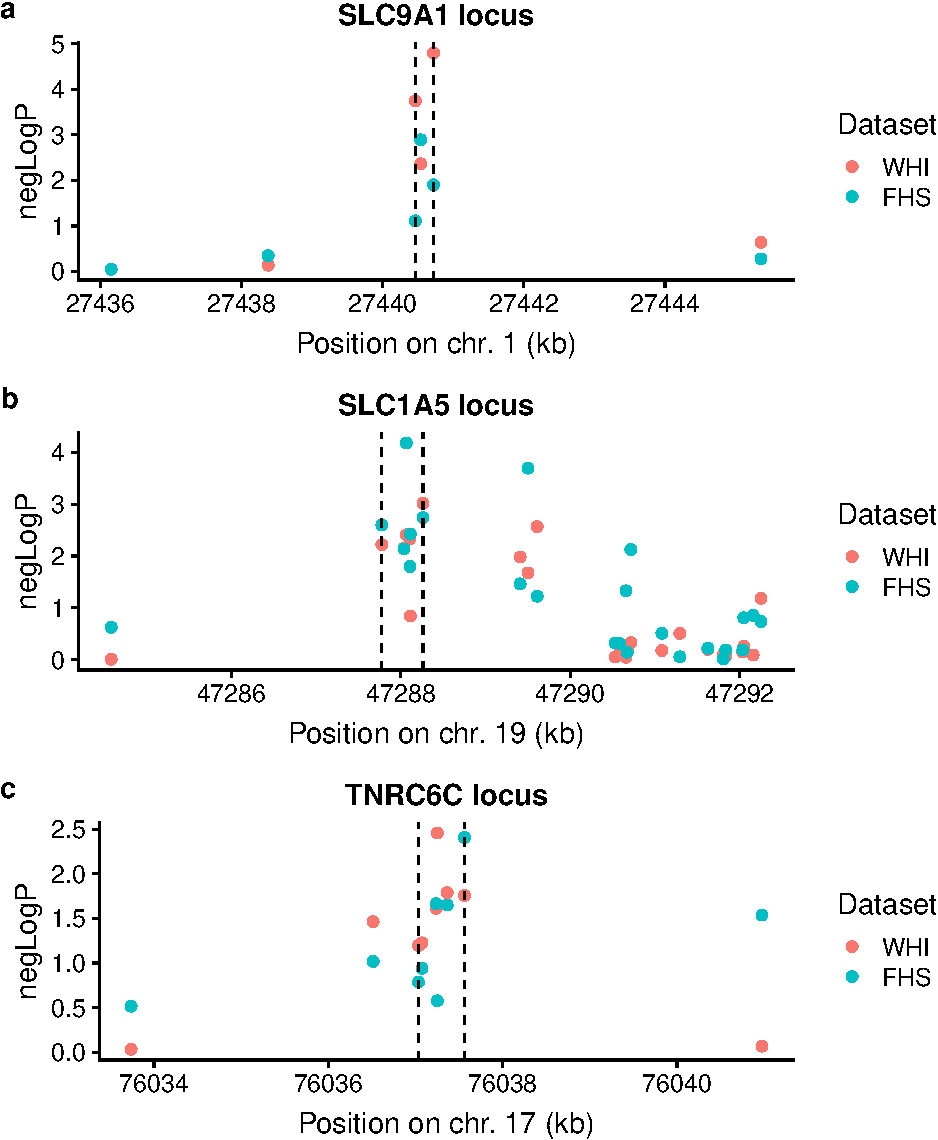
\includegraphics{../doc/module_ewas/figures/print-combp-plots-1.pdf}
\caption{\label{fig:print-combp-plots}DMRs identified by Comb-p in WHI and
validated in FHS at the (a) SLC9A1, (b) SLC1A5, and (c) TNRC6C loci.
Negative logarithms of EWAS p-values are shown as a function of the
genomic coordinate. EWAS p-values from WHI are in red and FHS in green.
Dotted lines demarcate the DMR boundaries.}
\end{figure}

\begin{figure}[htbp]
\centering
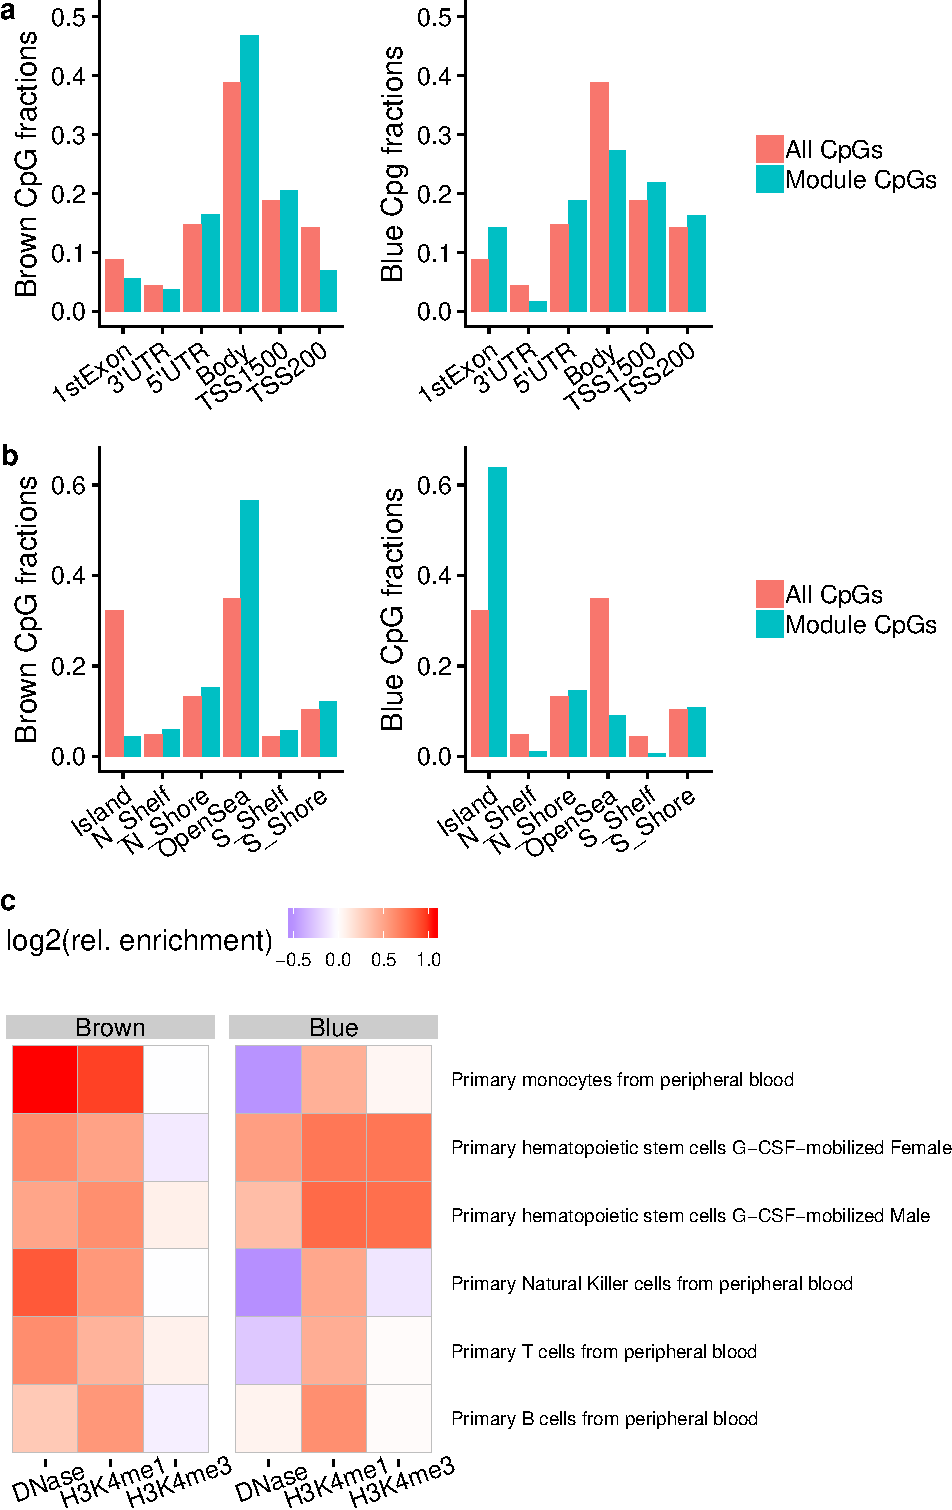
\includegraphics{../doc/module_ewas/figures/brown-and-blue-plots-1.pdf}
\caption{\label{fig:brown-and-blue-plots}Genomic and epigenomic annotations
of the brown and blue modules. a,b) Relative proportions of module CpGs
compared to the full set of CpGs tested, with respect to gene-based (a)
or CpG island-based (b) annotations (UTR = untranslated region; TSS\_X =
sites within X base pairs upstream of the gene transcription start
site). c) Cell type-specific enrichments based on Roadmap Epigenomics
datasets. Shown are relative enrichments of peaks (ratio of in-module
fraction to all-CpG fraction) for a given epigenetic mark across many
blood cell types, for each of the modules of interest.}
\end{figure}

\begin{figure}[htbp]
\centering
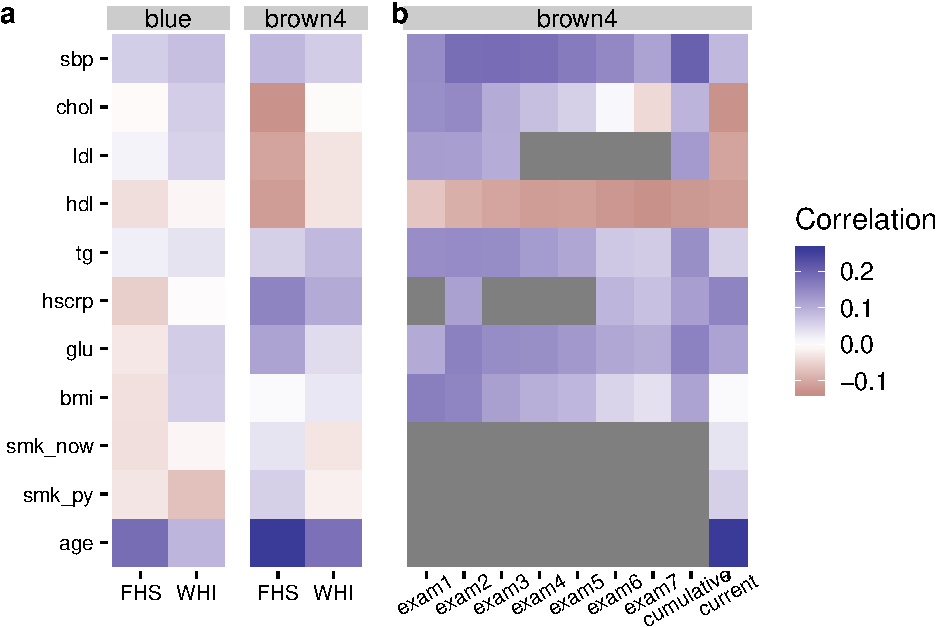
\includegraphics{../doc/module_ewas/figures/risk-factor-correlation-plots-1.pdf}
\caption{\label{fig:risk-factor-correlation-plots}Risk factor-module
relationships. (a) Pearson correlations between a series of traditional
cardiovascular risk factors and module eigenCpGs (blue and brown) are
shown in each study population. (b) Pearson correlations between
historical risk factor levels in FHS (across previous exams, x-axis) and
current brown module activation are shown. Grey panels indicate that
the risk factor in question was not available for the corresponding
exam.}
\end{figure}

\end{document}
